\documentclass[tikz,border=20pt]{standalone}
\usepackage{helvet}
\renewcommand{\familydefault}{\sfdefault}
\usepackage{tikz}
\usetikzlibrary{shapes,arrows,arrows.meta,positioning,calc,shapes.geometric,decorations.pathmorphing}

\definecolor{emeraldpine}{HTML}{1A4D3E}
\definecolor{harvardcrimson}{HTML}{A51C30}
\definecolor{ethdarkblue}{HTML}{1F407A}
\definecolor{ethpetrol}{HTML}{007A87}
\definecolor{ethbronze}{HTML}{B87333}
\definecolor{ink}{HTML}{1A202C}
\definecolor{cardbg}{HTML}{F8FAFC}
\definecolor{shadecolor}{HTML}{F4F6F9}
\definecolor{paleink}{HTML}{A0AEC0}

\begin{document}
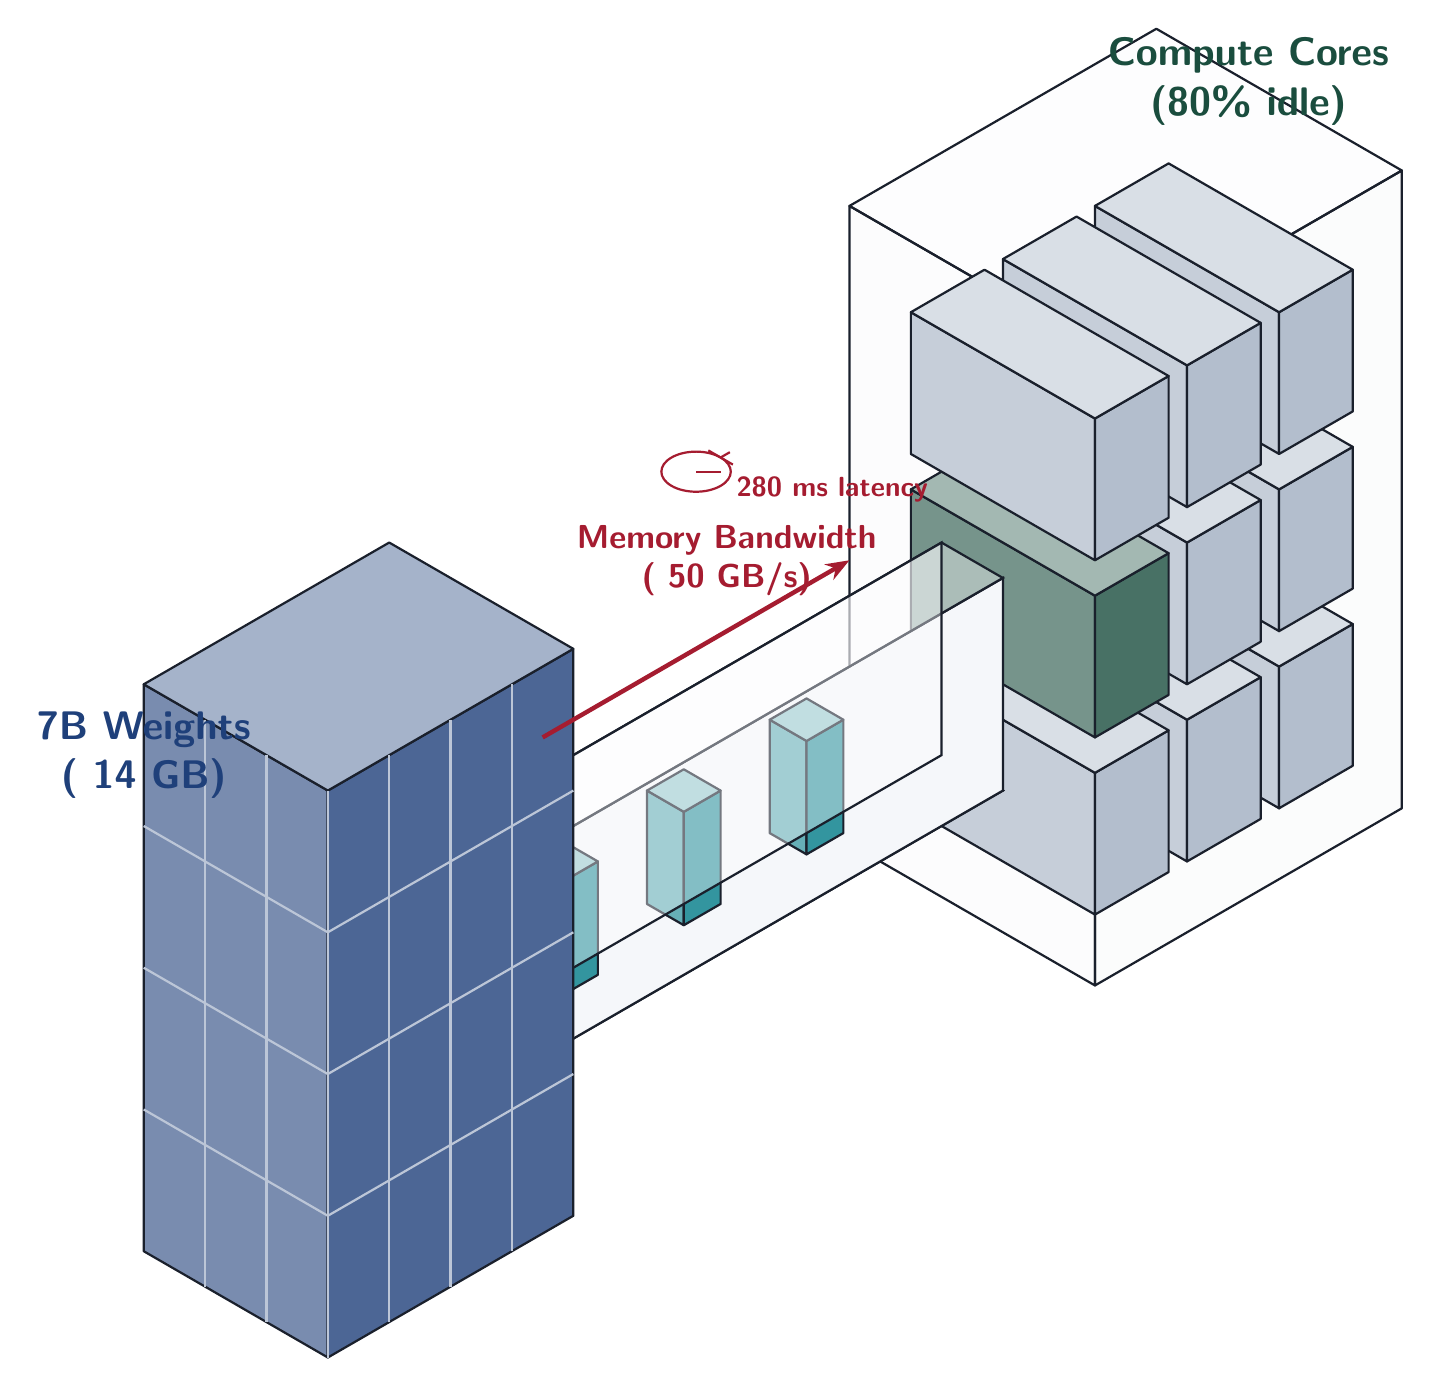
\begin{tikzpicture}[
    x={(0.866cm,-0.5cm)}, y={(0.866cm,0.5cm)}, z={(0cm,1cm)},
    font=\sffamily,
    scale=0.9
]

\def\drawbox#1#2#3#4#5#6#7#8{
    % Left face (y = #3)
    \filldraw[fill=#1!60, draw=ink, thick, fill opacity=#8, line join=round] (#2,#3,#4) -- (#2+#5,#3,#4) -- (#2+#5,#3,#4+#7) -- (#2,#3,#4+#7) -- cycle;
    % Right face (x = #2+#5)
    \filldraw[fill=#1!80, draw=ink, thick, fill opacity=#8, line join=round] (#2+#5,#3,#4) -- (#2+#5,#3+#6,#4) -- (#2+#5,#3+#6,#4+#7) -- (#2+#5,#3,#4+#7) -- cycle;
    % Top face (z = #4+#7)
    \filldraw[fill=#1!40, draw=ink, thick, fill opacity=#8, line join=round] (#2,#3,#4+#7) -- (#2+#5,#3,#4+#7) -- (#2+#5,#3+#6,#4+#7) -- (#2,#3+#6,#4+#7) -- cycle;
}

% === 1. COMPUTE CORES (Background/Right) ===
% We draw them first because they are at a higher y value
\drawbox{paleink}{-1}{12}{-0.5}{4}{5}{9}{0.05} % Outline enclosure, very faint

\node[emeraldpine, font=\bfseries\Large, align=center] at (1.0, 16.5, 9) {Compute Cores\\(80\% idle)};

% Draw 3x3 grid of cores. 
% y order: largest to smallest (back to front)
% z order: smallest to largest (bottom to top)
% x order: not varying here
\foreach \y in {15.5, 14.0, 12.5} {
    \foreach \z in {0, 2.5, 5} {
        \ifdim\y pt=12.5pt
            \ifdim\z pt=2.5pt
                % Active core
                \drawbox{emeraldpine}{-0.5}{\y}{\z}{3}{1.2}{2}{1.0}
            \else
                \drawbox{paleink}{-0.5}{\y}{\z}{3}{1.2}{2}{1.0}
            \fi
        \else
            \drawbox{paleink}{-0.5}{\y}{\z}{3}{1.2}{2}{1.0}
        \fi
    }
}

% === 2. PIPE (Back half) ===
% We draw the back faces of the pipe connecting DRAM to Compute
% Pipe from y=4 to y=12
\filldraw[fill=shadecolor!80, draw=ink, thick] (0.5, 4, 1.5) -- (1.5, 4, 1.5) -- (1.5, 12, 1.5) -- (0.5, 12, 1.5) -- cycle; % bottom
\filldraw[fill=shadecolor!90, draw=ink, thick] (1.5, 4, 1.5) -- (1.5, 4, 4.5) -- (1.5, 12, 4.5) -- (1.5, 12, 1.5) -- cycle; % back wall

% === 3. WEIGHT TILES (Inside Pipe) ===
% Draw weights from back to front (largest y to smallest y)
\drawbox{ethpetrol}{0.7}{9}{2.0}{0.6}{0.6}{1.6}{1.0}
\drawbox{ethpetrol}{0.7}{7}{2.0}{0.6}{0.6}{1.6}{1.0}
\drawbox{ethpetrol}{0.7}{5}{2.0}{0.6}{0.6}{1.6}{1.0}

% === 4. PIPE (Front half) ===
% Translucent front and top
\filldraw[fill=shadecolor!40, draw=ink, thick, fill opacity=0.4] (0.5, 4, 4.5) -- (1.5, 4, 4.5) -- (1.5, 12, 4.5) -- (0.5, 12, 4.5) -- cycle; % top
\filldraw[fill=shadecolor!20, draw=ink, thick, fill opacity=0.4] (0.5, 4, 1.5) -- (0.5, 4, 4.5) -- (0.5, 12, 4.5) -- (0.5, 12, 1.5) -- cycle; % front wall

% === 5. DRAM BANK (Foreground/Left) ===
\drawbox{ethdarkblue}{-0.5}{0}{0}{3}{4}{8}{1.0}

% Grid on DRAM
\foreach \z in {2,4,6} {
    \draw[ethdarkblue!30, thick] (-0.5, 0, \z) -- (2.5, 0, \z); % left face horizontal
    \draw[ethdarkblue!30, thick] (2.5, 0, \z) -- (2.5, 4, \z); % right face horizontal
}
\foreach \x in {0.5, 1.5, 2.5} {
    \draw[ethdarkblue!30, thick] (\x, 0, 0) -- (\x, 0, 8); % left face vertical
}
\foreach \y in {1, 2, 3} {
    \draw[ethdarkblue!30, thick] (2.5, \y, 0) -- (2.5, \y, 8); % right face vertical
}

% DRAM Label
\node[ethdarkblue, font=\bfseries\Large, align=center] at (-1.5, 1.0, 6) {7B Weights\\(~14 GB)};

% === 6. LABELS AND ANNOTATIONS ===
\node[harvardcrimson, font=\bfseries\large, align=center] at (1, 8, 6.5) {Memory Bandwidth\\(~50 GB/s)};
\draw[-{Stealth[length=3mm]}, harvardcrimson, ultra thick] (1, 5, 5.5) -- (1, 10, 5.5);

% Stopwatch (Adjusted coords for iso perspective)
\begin{scope}[shift={(1, 7.5, 8)}]
    \draw[harvardcrimson, thick, fill=white] (0,0) circle (0.4);
    \draw[harvardcrimson, thick] (0,0.4) -- (0,0.55);
    \draw[harvardcrimson, thick] (-0.2,0.4) -- (0.2,0.4);
    \draw[harvardcrimson, thick] (0,0) -- (0.2,0.2);
    \node[harvardcrimson, font=\bfseries, align=left, anchor=west] at (0.5, 0, 0) {280 ms latency};
\end{scope}

\end{tikzpicture}
\end{document}
